See \tabref{tab:rot-conic-params-sol}
and 
\figref{fig:chapters/11/11/4/5/1}.
In
\tabref{tab:rot-conic-params-sol}, $\vec{P}$ shifts the negative eigenvalue 
to get the hyperbola in standard form.
\begin{figure}[H]
	\begin{center} 
	    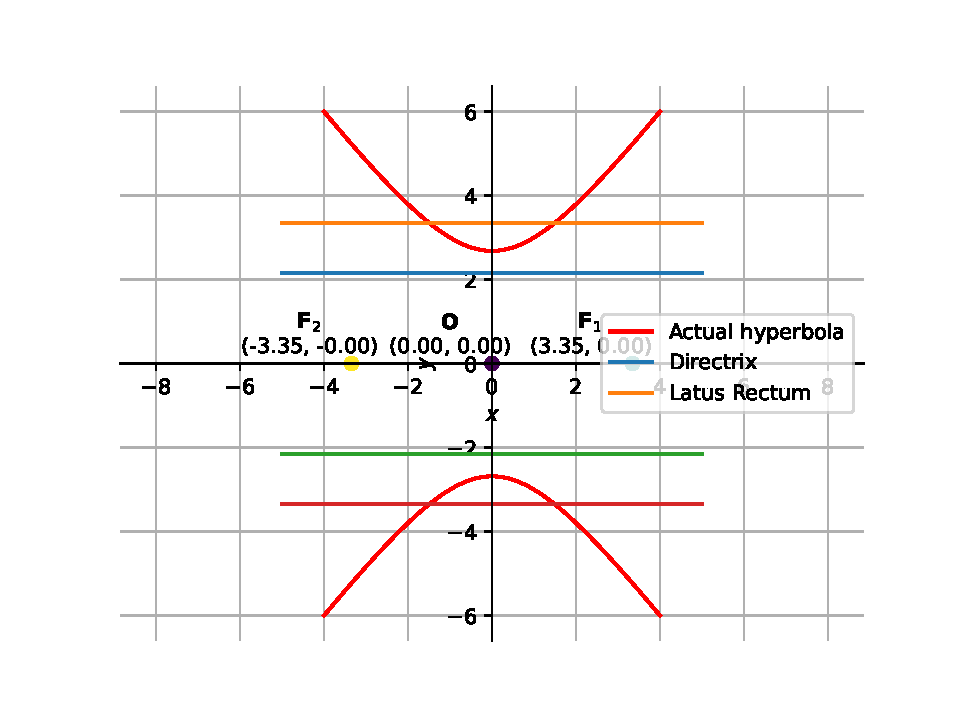
\includegraphics[width=0.75\columnwidth]{chapters/11/11/4/5/figs/fig.pdf}
	\end{center}
\caption{}
\label{fig:chapters/11/11/4/5/1}
\end{figure}

